\title{Study Guide for Midterm 2 for Calculus-Based Physics: Electricity and Magnetism}
\author{Dr. Jordan Hanson - Whittier College Dept. of Physics and Astronomy}
\date{\today}
\documentclass[10pt]{article}
\usepackage[a4paper, total={18cm, 27cm}]{geometry}
\usepackage{outlines}
\usepackage{graphicx}
\begin{document}
\maketitle

\begin{enumerate}
\item \textbf{Chapter 10: DC Circuits and Kirchhoff's Rules}
\begin{enumerate}
\item 
\begin{figure}[ht]
\centering
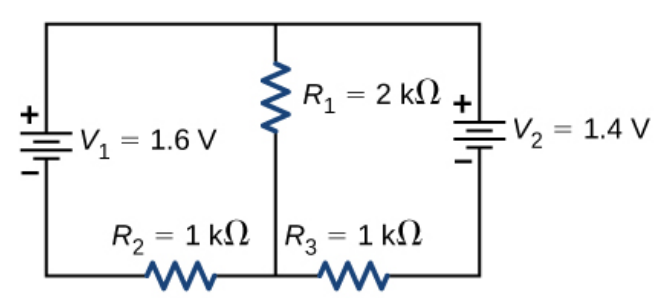
\includegraphics[width=0.4\textwidth]{circuit1.png}
\caption{\label{fig:circuit1} A circuit with five resistors powered by a battery with internal resistance.}
\end{figure}
What is the current flowing from the battery in Fig. \ref{fig:circuit1}?  What is the total power consumption? \\ \vspace{4cm}
\item 
\begin{figure}[ht]
\centering
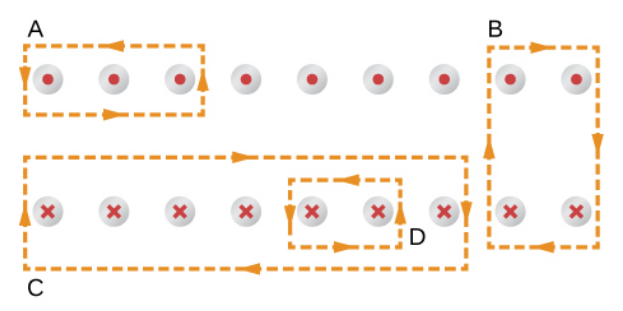
\includegraphics[width=0.4\textwidth]{circuit2.png}
\caption{\label{fig:circuit2} A circuit consisting of two batteries and five resistors.}
\end{figure}
Solve algebraiclly for the five currents in Fig. \ref{fig:circuit2}.  Remember to use the \textit{junction rule} and the \textit{loop rule.} \\ \vspace{4cm}
\item 
\begin{figure}[ht]
\centering
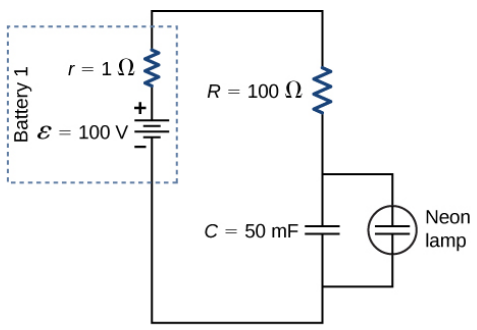
\includegraphics[width=0.3\textwidth]{circuit3.png}
\caption{\label{fig:circuit3} This type of circuit is called a relaxation oscillator.}
\end{figure}
Figure \ref{fig:circuit3} shows a \textit{relaxation oscillator}.  The RC circuit charges, and once the capacitor voltage reaches 50 V, the neon lamp lights and completely discharges the capacitor.  The process then repeats.  How long between neon lamp flashes? \\ \vspace{2cm}
\end{enumerate}
\item \textbf{Chapter 11: Magnetic forces and fields}
\begin{enumerate}
\item 
\begin{figure}[ht]
\centering
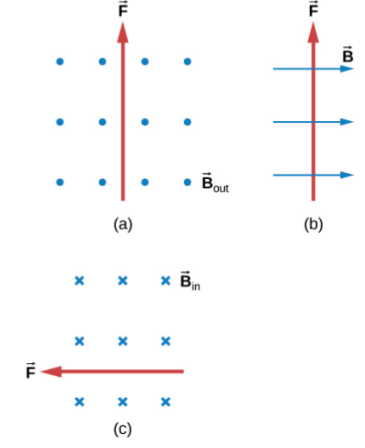
\includegraphics[width=0.3\textwidth]{lorentz1.png}
\caption{\label{fig:lorentz1} Each diagram depicts the force on a negatively-charged particle in a B-field.}
\end{figure}
Determine the velocity of a negatively-charged particle in Fig. \ref{fig:lorentz1} (a)-(c). \\ \vspace{1cm}
\item A cosmic-ray electron moves at $6 \times 10^6$ m/s perpendicular to Earth’s magnetic field at an altitude where the field strength is $1.0 \times 10^{-5}$ T. What is the radius of the circular path the electron follows?  Show that the \textit{angular velocity} $\omega$ of the electron around the magnetic field lines is related to the $q/m$ ratio by $\omega/B = q/m$. \\ \vspace{1.5 cm}
\item What is the maximum torque on a 150-turn circular loop of wire with radius 8.0 cm that carries a 50.0-A current in a 1.60 T B-field? \\ \vspace{2 cm}
\end{enumerate}
\item \textbf{Chapter 12: Sources of Magnetic Fields}
\begin{enumerate}
\item What is the magnetic field created by the loops in the previous problem, at the center of the loops?  What is the \textit{total} magnetic moment of the loops? \\ \vspace{1cm}
\item Using Amp\`{e}re's Law, re-derive the equation for a magnetic field due to a long staight wire.  Now model a lightning bolt as a long straight wire.  A typical current in a lightning bolt is $10^4$ A. Estimate the magnetic field 1 m from the bolt. \\ \vspace{1 cm}
\item
\begin{figure}
\centering
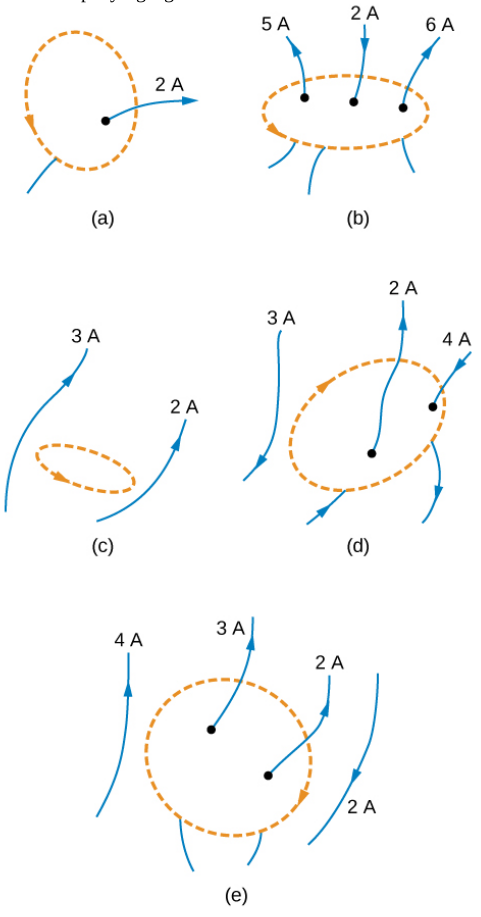
\includegraphics[width=0.3\textwidth,trim=0cm 0cm 0cm 0.25cm,clip=true]{amplaw.png}
\caption{\label{fig:amplaw} Several current arrangements with closed line integrals.}
\end{figure}
Evaluate $\oint \vec{B} \cdot d\vec{l}$ for cases (a)-(e) in Fig. \ref{fig:amplaw}.
\end{enumerate}
\end{enumerate}
\end{document}